\documentclass{standalone}

\usepackage{tikz,pgfplots}
\usepackage{amsmath,amssymb}
\usetikzlibrary{patterns}



\begin{document}
	
	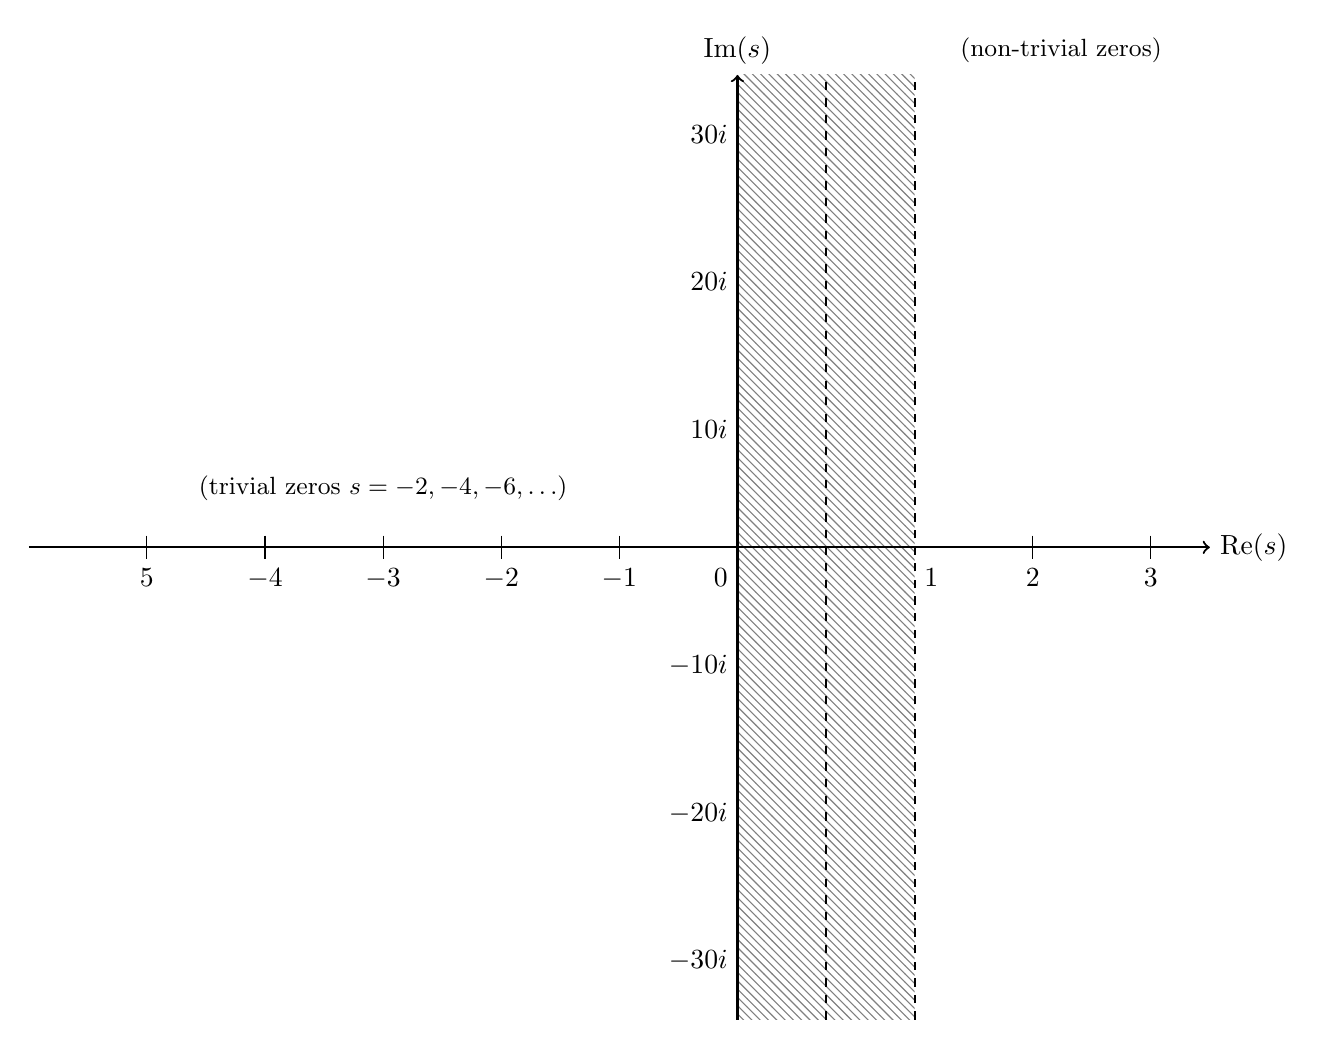
\begin{tikzpicture}[scale=1.5]
		\fill[pattern=north west lines, pattern color=gray] (0,-4) rectangle (1.5,4);
		\draw[thick,->] (-6,0) -- (4,0) node[right] {Re$(s)$};
		\draw[thick,->] (0,-4) -- (0,4) node[above] {Im$(s)$};
		\draw[dashed,thick] (1.5,-4) -- (1.5,4);
		\draw[dashed,thick] (0.75,-4) -- (0.75,4);
		\draw (0,-0.1) node[below left] {$0$};
		\draw (-1,0.1) -- (-1,-0.1) node[below] {$-1$};
		\draw (-2,0.1) -- (-2,-0.1) node[below] {$-2$};
		\draw (-3,0.1) -- (-3,-0.1) node[below] {$-3$};
		\draw (-4,0.1) -- (-4,-0.1) node[below] {$-4$};
		\draw (-5,0.1) -- (-5,-0.1) node[below] {$5$};
		\node at (2.74,4.4) [below] {\small (non-trivial zeros)};
		\node at (-3,0.5) {\small (trivial zeros $s = -2,-4,-6,\ldots)$};
		\node at (1.5,-0.1) [below right] {$1$};
		\draw (2.5,0.1) -- (2.5,-0.1) node[below] {$2$};
		\draw (3.5,0.1) -- (3.5,-0.1) node[below] {$3$};
		
		\node at (0,1) [left] {$10i$};
		\node at (0,2.25) [left] {$20i$};
		\node at (0,3.5) [left] {$30i$};
		
		\node at (0,-1) [left] {$-10i$};
		\node at (0,-2.25) [left] {$-20i$};
		\node at (0,-3.5) [left] {$-30i$};
	\end{tikzpicture}
	
	
	
	
	
	
	
	
	
	
	
\end{document} 